The last simulation performed by the authors had the goal of estimating the \textit{simulated cell growth inhibition percentage} of a treatment comprising both Cytarabine (Cyt) and Ibrutinib (Ibr). The authors were able to simulate a combined therapy without modifying the system of equations (which, in principle, is built to model the injections of a single type of drug) by modyfing the parameters of the model so that the combined therapy could be simulated as a single treatment (Fig. \ref{fig:combo}). In particular, the mixed treatment was obtained by combining Cyt High ($62.5$ mg/Kg of Cyt, $3 \cdot 10^{18}$ molecules of Cyt at each administration) and Ibr Low ($9$ mg/Kg of Ibr, $2.5 \cdot 10^{17}$ molecules of Ibr at each administration) for 8 days of treatment (5 days of treatment, 2 days of break, and another 3 days of treatment). This means injecting a total of $3.25 \cdot 10^{18}$ molecules at each administration. Since under these conditions Cyt represents approximately $92 \%$ of the total molecules, the combined treatment was parameterized by setting $\mu_{C} = (0.231 \cdot 0.92 + 0.116 \cdot 0.08) = 0.221$ and $\mu_{AC} = 0.012 + 0.0041 = 0.0161$. The simulation run with these parameters predicted a $95 \%$ cell growth inhibition. \par
\begin{figure}[htbp!]
    \centering
    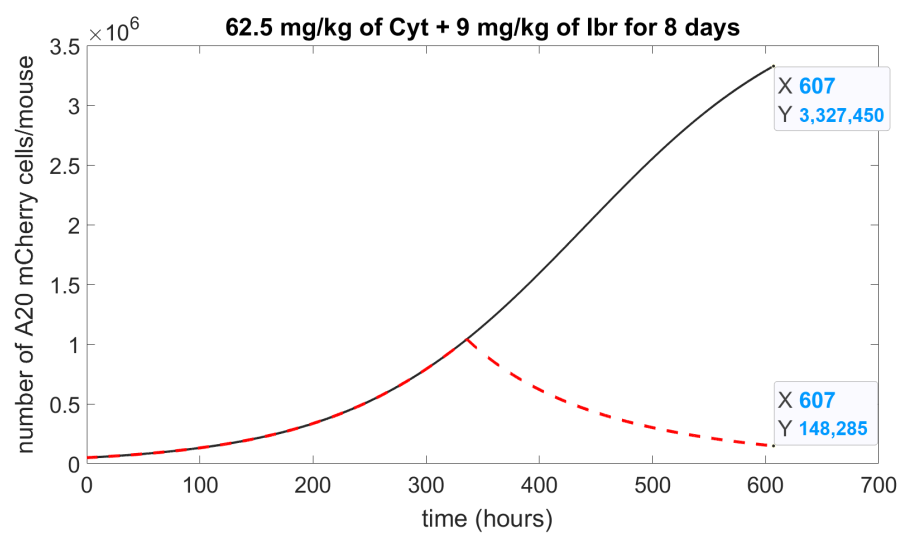
\includegraphics [scale = 0.27] {combined.png}
    \caption{Evolution of the system in the absence of treatment (black line) and with a combined protocol (red line)}
    \label{fig:combo}
\end{figure}
